% \documentclass[12pt]{article}

%%v helpful MIT exam schema, see http://www-math.mit.edu/~psh/exam/examdoc.pdf
 \documentclass[8pt]{exam} 
% \qformat{\textbf{Question \thequestion}\quad \thepoints\hfill } % Large depth to make space}
 \renewcommand{\thesubpart}{(\roman{subpart})}
 \renewcommand{\subpartlabel}{\thesubpart}
 \footer{}{}{Page \thepage\ de \numpages}
\addpoints
% \pointsinmargin
% \boxedpoints
\renewcommand{\questionshook}{\setlength{\itemsep}{0.2cm}}
\renewcommand{\partshook}{
	\setlength{\itemsep}{0.1cm}
}

\usepackage{cmbright}

\pagestyle{empty} %for handouts
\addtolength{\jot}{2em} % this makes all formulae a bit more spaced vertically for handouts
\setlength{\parindent}{0pt} %we're not writing a novel
%\renewcommand{\arraystretch}{2} %makes tables taller, so easier to write in

\usepackage[fleqn]{amsmath}
\usepackage{amssymb} %standard classy maths symbols
\usepackage[a4paper, margin=1in]{geometry} %makes it easy to specify where to put stuff on the page

\usepackage{siunitx} %v handy way of getting SI units to typeset correctly...
% \sisetup{locale = FR} %... and now it will use a comma for decimals

\usepackage[utf8]{inputenc}

% \usepackage[french]{babel} % frenchify everything (e.g. a Table becomes a Tableau)
% \usepackage{lmodern} % font with nicer French characters than standard
% \usepackage{textcomp} % and more help for special characters

\usepackage{tcolorbox} % basic but good package for boxes around text
\tcbset{colback=black!5!white}
% \usepackage{color} % colours
%\newcommand{\fillin}{\color{black!1!white}} %makes the text disappear
%\definecolor{fillin}{rgb} {1.00,1.00,1.00}
%\renewcommand{\fillin}{\color{blue}} \definecolor{fillin}{rgb} {0.00,0.00,1.00} %makes the filling in text appear (in blue)

\usepackage{enumitem} % can change the labels on lists, items, enumerates
\usepackage{setspace}

\usepackage{tikz, pgfplots} % interval diagrams, sets, etc.
\usetikzlibrary{calc,trees,positioning,arrows,fit,shapes,angles,quotes}

\newcommand\TikCircle[1][2.5]{\tikz[baseline=-#1]{\draw[thick](0,0)circle(3mm)[radius=#1mm];}}

\begin{document}


\begin{minipage}{0.7\textwidth}
\begin{tcolorbox}[width=10cm]
Reminder, from p. 32 of CRM. \\
\textbf{The sine rule :}

\

$\displaystyle \frac{a}{\sin(\alpha)} = \frac{b}{\sin(\beta)} = \frac{c}{\sin(\gamma)}$
\vspace{-20mm}

\hfill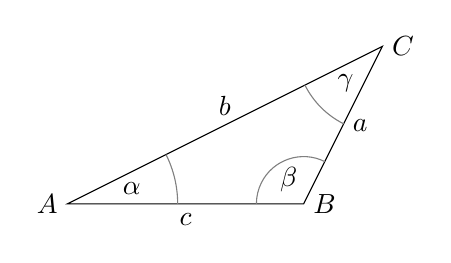
\begin{tikzpicture}

  \coordinate (A) at (0,0);
  \coordinate (B) at (3,0);
  \coordinate (C) at (4,2);

  \draw (C) node[right] {$C$} -- node[right]{$a$}  (B) node[right] {$B$} --  node[below] {$c$} (A) node[left] {$A$}  -- node[above] {$b$} cycle;

\pic [angle radius=6mm, draw=gray, "$\beta$" ] {angle=C--B--A};
\pic [angle radius=11mm, draw=gray,"$\gamma$"] {angle=A--C--B};
\pic [angle radius=14mm, draw=gray, "$\alpha$" ] {angle=B--A--C};

\end{tikzpicture}

\vspace{-2mm}
\end{tcolorbox}
\end{minipage}
\begin{minipage}{0.3\textwidth}
\textbf{Name:} \dotfill

\vspace{8mm}
\dotfill
\end{minipage}

\begin{questions}


\question[5] $\triangle XYZ$ is right-angled in $X$ with $\hat{Y} = 40^\circ$. Given that $\overline{XY} = 12$, calculate $\overline{YZ}$ to 1 d.p.
\fillwithdottedlines{70mm}

\question[5] \textbf{Solve} the following triangle (1 d.p.). \hfill \emph{This means find all angles and lengths.}
\vspace{-3mm}

\begin{minipage}{0.6\textwidth}
\fillwithdottedlines{5cm}
\end{minipage}
\hfill
\begin{minipage}{0.3\textwidth}
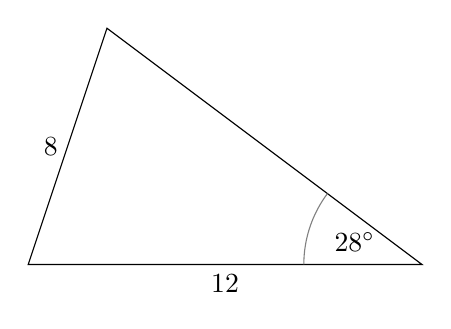
\begin{tikzpicture}

  \coordinate (A) at (0,0);
  \coordinate (B) at (5,0);
  \coordinate (C) at (1,3);

  \draw (C) -- (B) -- node[below]{12}  (A) -- node[left]{8} cycle;

\pic [angle radius=15mm, draw=gray, "$28^\circ$" ] {angle=C--B--A};
%\pic [angle radius=10mm, draw=gray,"$A$"] {angle=A--C--B};
%\pic [angle radius=12mm, draw=gray, "$80^\circ$" ] {angle=B--A--C};

\end{tikzpicture}
\end{minipage}

\vspace{-3mm}
\fillwithdottedlines{\stretch{1}}


\question[0] \textbf{Bonus.} Solve $\sin (\theta) = 1$. \hfill \emph{Work on the back.}
\end{questions}


\begin{tcolorbox}

\textbf{Name of examiner:}

\begin{center}
\gradetable[h][questions]
\end{center}

\end{tcolorbox}

\end{document}